\documentclass{beamer}
\usepackage[utf8]{inputenc}

\usetheme{Madrid}
\usecolortheme{default}
\usepackage{amsmath,amssymb,amsfonts,amsthm}
\usepackage{txfonts}
\usepackage{tkz-euclide}
\usepackage{listings}
\usepackage{adjustbox}
\usepackage{array}
\usepackage{tabularx}
\usepackage{gvv}
\usepackage{lmodern}
\usepackage{circuitikz}
\usepackage{tikz}
\usepackage{graphicx}

\setbeamertemplate{page number in head/foot}[totalframenumber]

\usepackage{tcolorbox}
\tcbuselibrary{minted,breakable,xparse,skins}



\definecolor{bg}{gray}{0.95}
\DeclareTCBListing{mintedbox}{O{}m!O{}}{%
	breakable=true,
	listing engine=minted,
	listing only,
	minted language=#2,
	minted style=default,
	minted options={%
		linenos,
		gobble=0,
		breaklines=true,
		breakafter=,,
		fontsize=\small,
		numbersep=8pt,
		#1},
	boxsep=0pt,
	left skip=0pt,
	right skip=0pt,
	left=25pt,
	right=0pt,
	top=3pt,
	bottom=3pt,
	arc=5pt,
	leftrule=0pt,
	rightrule=0pt,
	bottomrule=2pt,
	toprule=2pt,
	colback=bg,
	colframe=orange!70,
	enhanced,
	overlay={%
		\begin{tcbclipinterior}
			\fill[orange!20!white] (frame.south west) rectangle ([xshift=20pt]frame.north west);
	\end{tcbclipinterior}},
	#3,
}
\lstset{
	language=C,
	basicstyle=\ttfamily\small,
	keywordstyle=\color{blue},
	stringstyle=\color{orange},
	commentstyle=\color{green!60!black},
	numbers=left,
	numberstyle=\tiny\color{gray},
	breaklines=true,
	showstringspaces=false,
}
%------------------------------------------------------------
%This block of code defines the information to appear in the
%Title page
\title %optional
{2.4.29}

%\subtitle{A short story}

\author % (optional)
{Nipun Dasari - EE25BTECH11042}



\begin{document}
	
		\frame{\titlepage}
	\begin{frame}{Question}
	The points $\vec{A}\brak{2, 9}$, $\vec{B}\brak{a, 5}$ and $\vec{C}\brak{5, 5}$ are the vertices of a triangle $\vec{ABC}$ right angled
	at $\vec{B}$. Find the values of a and hence the area of $\Delta\vec{ABC}$. \\
	\end{frame}

	
\begin{frame}{Theoretical Solution}
Given the points A, B and C, also consider $\vec{c}$ to be vector opposite to side AB and $\vec{b}$, $\vec{a}$ similarly

\begin{align}
	\vec{A} = \begin{myvec}{2\\9} \end{myvec} , \vec{B} = \begin{myvec}{a\\5} \end{myvec}, \vec{C} = \begin{myvec}{5\\5} \end{myvec}
\end{align}
Since the sides c and a are perpendicular their inner product will be 0\\
Take the inner product of $\vec{c}$ and $\vec{a}$\\
Vector $\vec{c}$:
\begin{align}
	\vec{c} = \vec{A}-\vec{B} = \begin{myvec}{2 -a\\9 - 5} \end{myvec} = \begin{myvec}{2 -a\\4} \end{myvec}
\end{align}
Vector $\vec{a}$:
\end{frame}
\begin{frame}{Theoretical Solution}
\begin{align}
	\vec{a} = \vec{B}-\vec{C} = \begin{myvec}{a - 5\\5 - 5} \end{myvec} = \begin{myvec}{a - 5 \\0} \end{myvec}
\end{align}
Orthogonality $\implies$ matrix product is zero :
\begin{align}
	\vec{c}^T\vec{a} = \begin{myvec}{2 -a & 4} \end{myvec}\begin{myvec}{a - 5 \\0} \end{myvec} = \brak{2-a}\brak{a-5} = 0
\end{align}
So \brak{2-a}\brak{5-a} = 0 $\implies$ $a = 2$ or $a = 5$.\\
$a = 5$ make $\vec{B}$=$\vec{C}$. $\therefore a =2$  \\
We can compute area using cross product formula
\end{frame}
\begin{frame}{Theoretical Solution}
\begin{align}
	\Delta = \frac{1}{2}\norm{\vec{c}\times\vec{a}} \label{eq:0.5}
\end{align}
The general cross product of two vectors is defined as:
\begin{align}
	\vec{A}\times\vec{B} = \begin{myvec}{|\vec{A}_{23} & \vec{B}_{23}|\\|\vec{A}_{31} & \vec{B}_{31}|\\|\vec{A}_{12} & \vec{B}_{12}|} \end{myvec} \label{0.6}
\end{align}
The vectors in 3-D space look like
\begin{align}
	\vec{c} = \begin{myvec}{0\\4\\0} \end{myvec}
\end{align}
\end{frame}
\begin{frame}{Theoretical Solution}
\begin{align}
	\vec{a} = \begin{myvec}{-3 \\0\\0} \end{myvec}
\end{align}
\begin{align}
	\vec{c}_{31} \text{ } \vec{a}_{31}| = |\begin{mydet}{0 & 0\\ 0 & -3} \end{mydet} = 0
\end{align}
\begin{align}
	|\vec{c}_{23} \text{ } \vec{a}_{23}| = \begin{mydet}{4 & 0\\ 0 & 0} \end{mydet} = 0
\end{align}
\begin{align}
	|\vec{c}_{12} \text{ } \vec{a}_{12}| = \begin{mydet}{0 & 4\\ -3 & 0} \end{mydet} = 12
\end{align}
\end{frame}
\begin{frame}{Theoretical Solution}
	
By \eqref{0.6}:
\begin{align}
	\vec{c}\times\vec{a} = \begin{myvec}{0 \\ 0 \\ 12} \end{myvec}
\end{align}
\begin{align}
	\norm{\vec{c}\times\vec{a}} = 12
\end{align}



Using \eqref{eq:0.5}
\begin{align}
	\therefore	\Delta = \frac{1}{2}\norm{\vec{c}\times\vec{a}} = 6
\end{align}
Thus area of triangle is $6$\\

	\end{frame}

	\begin{frame}[fragile]
	\frametitle{C Code- Triangle Area function }
	
	\begin{lstlisting}
// triangle.c
#include <math.h>

float triangle_area(float ax, float ay, float bx, float by, float cx, float cy) {
	float area = fabs(ax*(by-cy) + bx*(cy-ay) + cx*(ay-by)) / 2.0;
	return area;
}
	\end{lstlisting}
\end{frame}

\begin{frame}[fragile]
	\frametitle{Python Code using shared output}
	\begin{lstlisting}
import ctypes
import numpy as np
import matplotlib.pyplot as plt

# Load the shared C library
lib = ctypes.CDLL("./trianglearea.so")
lib.triangle_area.argtypes = [ctypes.c_float, ctypes.c_float,
ctypes.c_float, ctypes.c_float,
ctypes.c_float, ctypes.c_float]
lib.triangle_area.restype = ctypes.c_float

# Vertices
A = (2, 9)
B = (2, 5)
C = (5, 5)
	\end{lstlisting}
\end{frame}
\begin{frame}[fragile]
	\frametitle{Python Code using shared output}
	\begin{lstlisting}		
# Call C function
area = lib.triangle_area(A[0], A[1], B[0], B[1], C[0], C[1])
print("Area of triangle ABC (from C):", area)

# Plot triangle
x = [A[0], B[0], C[0], A[0]]
y = [A[1], B[1], C[1], A[1]]

plt.plot(x, y, 'bo-')
plt.text(A[0], A[1], "A(2,9)", fontsize=10, ha="right")
plt.text(B[0], B[1], "B(2,5)", fontsize=10, ha="right")
plt.text(C[0], C[1], "C(5,5)", fontsize=10, ha="right")
plt.title("Right Triangle ABC")
plt.grid(True)
plt.axis("equal")
plt.show()
	\end{lstlisting}
\end{frame}
\begin{frame}[fragile]
	\frametitle{Python Code using shared output}
	\begin{lstlisting}
		# Plotting
		plt.figure(figsize=(6, 6))
		plt.scatter(A[0], A[1], color='red', label='A(5,1)')
		plt.scatter(B[0], B[1], color='blue', label='B(-1,5)')
		plt.scatter(midpoint[0], midpoint[1], color='black', label='Midpoint')
		
		# Perpendicular bisector line
		plt.plot(x_vals, y_vals, 'g--', label='3x = 2y (Perp. bisector)')
		
		# Mark example points
		for p in points_to_check:
		plt.scatter(p[0], p[1], label=f"Point {p}")
	\end{lstlisting}
\end{frame}
\begin{frame}[fragile]
	\frametitle{Python Code}
	\begin{lstlisting}
import numpy as np
import matplotlib.pyplot as plt

# Vertices
A = np.array([2, 9])
B = np.array([2, 5])
C = np.array([5, 5])

# Check right angle at B using dot product
AB = A - B
BC = C - B
print("Dot product AB·BC =", np.dot(AB, BC))

	\end{lstlisting}
\end{frame}

\begin{frame}[fragile]
	\frametitle{Python Code}
	\begin{lstlisting}
if np.dot(AB, BC) == 0:
print("Right angle at B ✅")


area = abs(np.linalg.det(np.array([
[A[0], A[1], 1],
[B[0], B[1], 1],
[C[0], C[1], 1]
]))) / 2
print("Area of triangle ABC (Python):", area)

# Plot
x = [A[0], B[0], C[0], A[0]]
y = [A[1], B[1], C[1], A[1]]
	\end{lstlisting}
\end{frame}

\begin{frame}[fragile]
	\frametitle{Python Code}
	\begin{lstlisting}
plt.plot(x, y, 'ro-')
plt.text(A[0], A[1], "A(2,9)", fontsize=10, ha="right")
plt.text(B[0], B[1], "B(2,5)", fontsize=10, ha="right")
plt.text(C[0], C[1], "C(5,5)", fontsize=10, ha="right")
plt.title("Right Triangle ABC (Pure Python)")
plt.grid(True)
plt.axis("equal")
plt.show()
	\end{lstlisting}
\end{frame}

\begin{frame}{Plot by python using shared output from c}
	\begin{center}
	\begin{figure}[H]
		\centering
		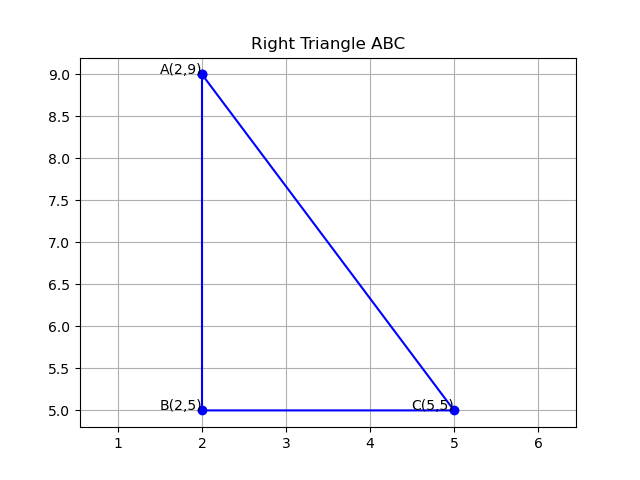
\includegraphics[width = 0.6\columnwidth]{figs/Figure_1.png}
		\caption*{}
		\label{}
	\end{figure}
	\end{center}
\end{frame}

\begin{frame}{Plot by python only}
	\begin{center}
		\begin{figure}[H]
			\centering
			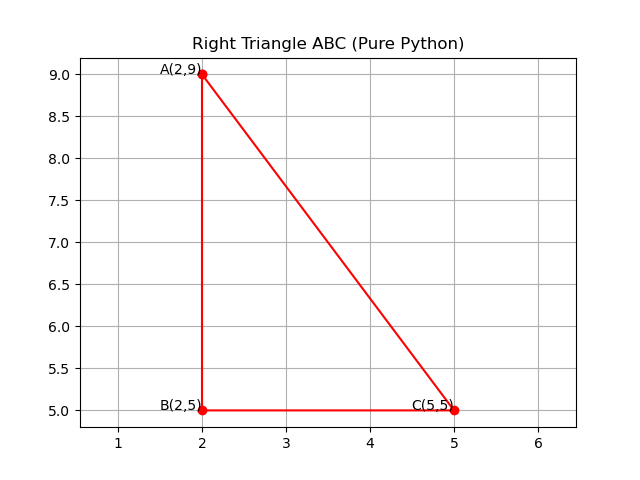
\includegraphics[width = 0.6\columnwidth]{figs/Figure_2.png}
			\caption*{}
			\label{}
		\end{figure}
	\end{center}
\end{frame}
\end{document}
